\section{Workflow and \gaia{} Compiler}
\label{sec:workflow}

In this section, we first put things together, introducing the workflow of \gaia{}, then discuss the implementation of a highly modular compiler of \gaia{}.

\begin{figure}[h]
  \centering
  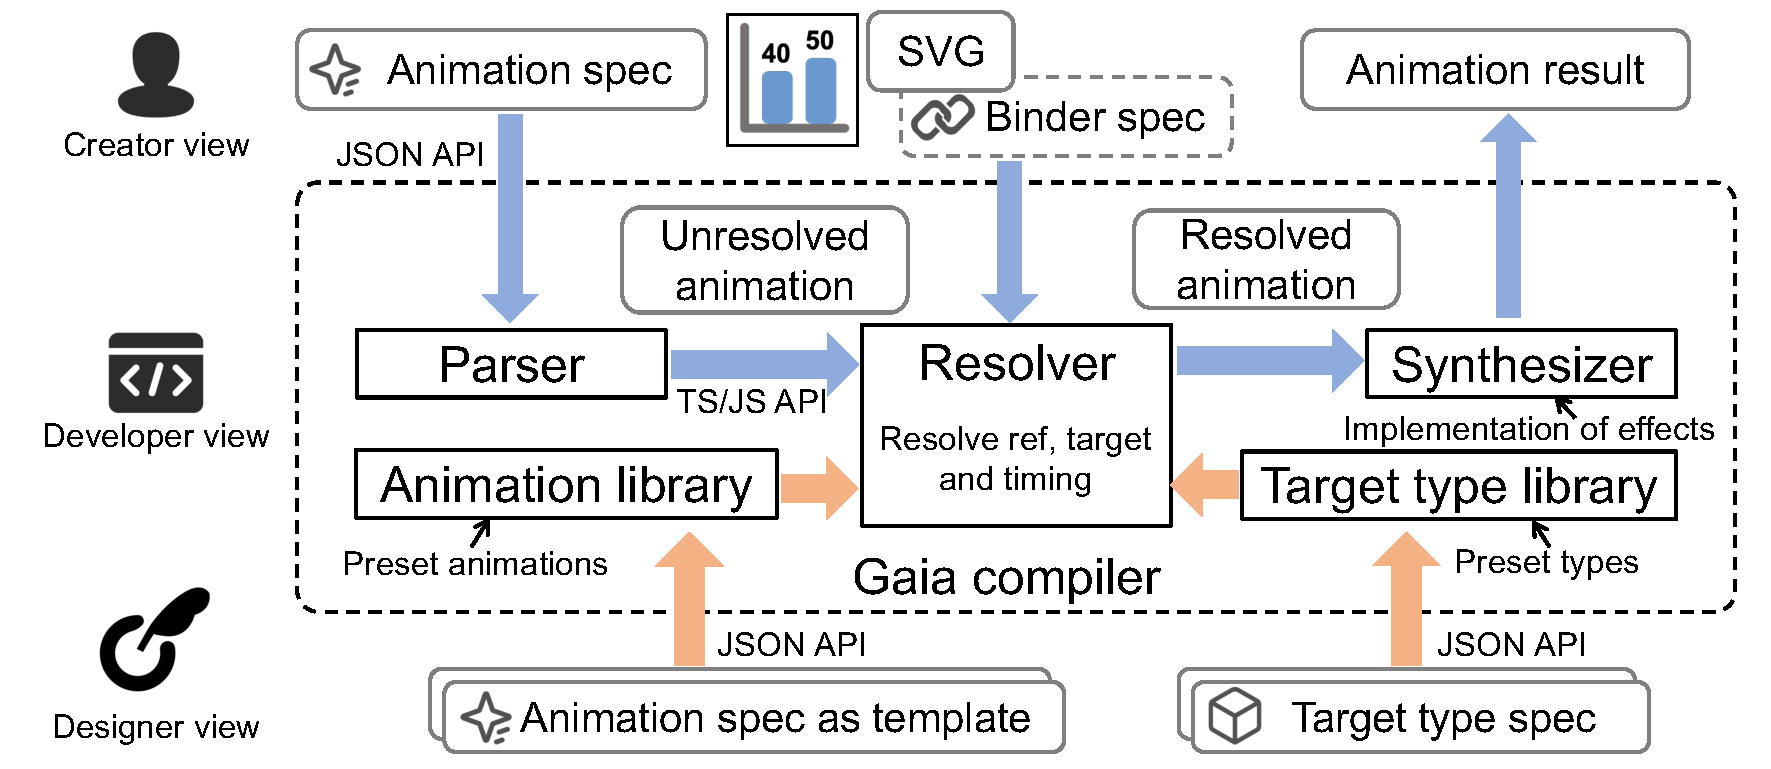
\includegraphics[width=\linewidth]{figs/workflow.pdf}
  \caption{Workflow of \gaia{} from three views and implementation of \gaia{} compiler.}
%  \Description{}
  \label{fig:workflow}
\end{figure}

\subsection{Workflow of \gaia{}}

% As shown in \autoref{fig:workflow}, the workflow is threefold:
% animations can be applied to SVGs to define animation actions

As shown in \autoref{fig:workflow}, the workflow of \gaia{} has three views.

\begin{enumerate}
\item \textbf{Creator view}.
For end users whose expectation is a visible animation, \gaia{} hides the most complexity of designing detailed animations and implementing effects. 
They only need to specify their top-level animation spec and provide an infographic with declared types. 
Creators can be human users or tools that use \gaia{} to create animations.

\item \textbf{Designer view}.
Animation design experts can design target types and provide high-quality animation templates for them.
They don't need to care about the structure of the real infographic, nor be aware of the implementation. 
Instead, they simply focus on animations from themselves or other designers using high-level grammar, creating animations that are consistent in style and mood, and clear in meaning.

\item \textbf{Developer view}.
Developers need to implement basic animation effects and serve them as code-native \aniclass{}es. In our implementation of \gaia{}'s compiler, this work is minimized as the modular design (\autoref{ssec:compiler}).
Most of the \gaia{} compiler components don't require any change when adding effects.

\end{enumerate}

The border between creators, designers and developers is not clear-cut. Creators can also build their templates and types for convenience. 
Developers can also define \aniclass{}es, like designers, with TS/JS API.
Anyway, Gaia decouples the final creator of the animation, the professional designer of the animation template and the developer of the animation effect from each other, so that each part can be developed and changed separately, and the complexity of other domains can be hidden. 
This stems from Gaia's unique reusability and extensibility.


\subsection{\gaia{} Compiler Prototype}
\label{ssec:compiler}

\gaia{} frameworks need to provide consistent, efficient APIs for different users, while ensuring reusability and extensibility at the framework level.
We implemented a prototype of \gaia{} compiler and published it as a library.
The middle part of \autoref{fig:workflow} illustrates the pipeline of the compiler.
For the creator side, the compiler takes the animation spec and the infographic as input and outputs the animation result.
The pipeline involves three steps: \textbf{parsing}, \textbf{resolving} and \textbf{synthesizing}. 
First, for any high-level spec written in JSON, a parser is used to transform it into a \gaia{} internal object using TS/JS API.
The animation spec, in this step, will form a data structure called \textbf{unresolved animation}, which is a tree-like structure.
Next, a virtual target model is created with the declared types and the given SVG.
Then, the compiler resolves the animation, linking the animations declared with \code{ref} from the library, resolving selected targets on the virtual model, and computing duration.
So far, this \textbf{resolved animation} does not rely on any specific implementation details but contains all the information for the animation.
It can be returned to the user layer for preview, debugging, or building UI (if the creator is a tool using \gaia{}).
Finally, the compiler synthesizes the resolved animation and creates the animated instance with the implementation of effects (which are tackled by developers).

It is important to note that \gaia{} provides a complete end-to-end system for creators and designers, but each component used in the compiler pipeline can be replaced.
For instance, an alternate parser can be supplied so that new features of JSON spec, or other high-level grammars, can be hired to construct unresolved animation objects.
As another example, the synthesizer can have a different implementation of the same \aniclass{} to support different element types, such as HTML and SVG, in a seamless way for high-level spec users.
Besides, the animation and target type library can be remotely stored and fetched.
We implemented a RESTful server as a remote library for internal use, which allows users to upload and download animation specs and target type specs.
